%----------------------------------------------------------------------------------------
% Corporate Design 2016 Presentation
%----------------------------------------------------------------------------------------
% Last update 22.11.2017
%
% Changelog:
%   22.11.2017: changed style of numbered slides
%   21.11.2017: added \toogleFooter to hide/show footer on teh following slides
%   30.06.2017: added \enum{#number} to link to an enuemrate item
%   20.04.2017: added numbered option too show slide number at bottom-right, also an example for usage in individual footers, i.e. with \setFooter
%   30.11.2016: improved documentation of titlepage picture and some minor changes
%   28.11.2016: fix for [t] alignment to \frame
%   23.11.2016: FKR release version
%   21.11.2016: improvements for adaptability to institute-level
%   18.11.2016: initial version
%
% For questions or bug reports
% mailto: mirco.altenbernd@ians.uni-stuttgart.de
%
%----------------------------------------------------------------------------------------
% Obligatory settings and includes
%------------------------------------------------------------------------------
\pdfminorversion=4
\documentclass[11pt,aspectratio=1610]{beamer}
\usepackage{multicol}
\usepackage{mathtools} 
\usepackage{mathrsfs} % used for mathscr
\newcommand{\FF}{\mathcal{F}}
\newcommand{\HH}{\mathscr H}
\newcommand{\LL}{\mathscr L}
\newcommand{\ii}{i}


\usepackage{amsmath,amssymb,amsthm}
\usepackage{pstricks,pst-node,pst-coil,pst-plot,pstricks-add}
\usepackage{geometry,epsfig}
\usepackage{bbm}
\usepackage{bm} %für \boldsymbol
\usepackage{cite}
\usepackage{xcolor} % Für Farbe
\usepackage{empheq} % Für Boxen



\newcommand{\C}{\mathbb{C}} % komplexe
\newcommand{\K}{\mathbb{K}} % komplexe
\newcommand{\R}{\mathbb{R}} % reelle
\newcommand{\Q}{\mathbb{Q}} % rationale
\newcommand{\Z}{\mathbb{Z}} % ganze
\newcommand{\N}{\mathbb{N}} % natuerliche
\DeclareMathOperator*{\esssup}{ess\,sup}
\newcommand{\B}[1]{ \textbf{#1}}


%\newcommand{\begin{proof}}{\textit{Proof. }}	%für Beweise	
%\newcommand{\end{proof}inalign}{\tag*{$\blacksquare$}} %eproof in align Umgebung nach rechts
%\newcommand{\end{proof}}{\hfill $\blacksquare$}	

\DeclareRobustCommand{\rchi}{{\mathpalette\irchi\relax}}
\newcommand{\irchi}[2]{\raisebox{\depth}{$#1\chi$}} %richtiges Chi
\newcommand{\intd}{\int \hspace{-1.5mm} d} %\int dx richtig plaziert
\newcommand{\all}{\quad \text{for all} \: \,} %Abkürzung von für alle
\newcommand{\Ima}{\operatorname{Im}}
\newcommand{\Rea}{\operatorname{Re}}

\renewcommand{\baselinestretch}{1.1}
\renewcommand{\qedsymbol}{\rule{1.3mm}{2.6mm}}


%
%------------------------------------------------------------------------------
% Basic slide layout configuration
%
% Important: remove all auxiliary files before recompilation when switching
%            from english (the default) to german and vice versa
%------------------------------------------------------------------------------
% \usetheme{fbm2016}                  % english talk
%\usetheme[simtech]{fbm2016}         % english, with additional SimTech logo
%\usetheme[german]{fbm2016}          % german
%\usetheme[numbered]{fbm2016}        % add slide count to the bottom right, only if '\setFooter' is not used. Otherwise see example in '\setFooter' to obtain similar results
\usetheme[german,simtech]{fbm2016}  % german, with SimTech logo
%
% feel free to implement GRK 1838 etc., by cloning the SimTech option
%
%------------------------------------------------------------------------------
% additional packages, anything beamer-compatible is allowed
%------------------------------------------------------------------------------
\usepackage{amsmath}  % just an example
\usepackage{amssymb}  % just an example
\usepackage{amsthm}   % just an example
%
%------------------------------------------------------------------------------
% Personalisation of title page, and inividual footers on all subsequent slides
%------------------------------------------------------------------------------

\title{Project 2: Time dependent heat equation with a source}
\subtitle{\small{Scientific Computing}
}
\author{V.~Ku{\ss}maul, N.~Thorin}
\date{\, }
% subtext below "Uni-Stuttgart" logo on frontpage
\setLogoText{Department of Mathematics}
% background image for titlepage, with and without size
% \setTitlePic{decay.png}
% \defTitlePic{\includegraphics[height=6cm]{titlepic.jpg}}
% complete removal of the image
\defTitlePic{}


% Define an individual footer. If not set a default footer is used which depends on the used beamer options: simtech, german, numbered
% Up to three optional logos/URLs/names in all footers of subsequent slides,
% please only edit lines marked as %%%%.
 \setFooter{
 	\vspace*{1cm} % for alignment issues: otherwise the content does not recognize the footer
   \begin{tikzpicture}[remember picture,overlay]
     % horizontal line
     \ifnum\thepage>1\draw (0.5,1) node(a) {} (15.5,1) node(b) {}; \draw[CD01!40] (a.east) -- (b.west);\fi
      %left aligned footer-content
      \node[anchor=south west, align=left, yshift=0.01\paperwidth, xshift=0.036\paperwidth] at (current page.south west) {
       %\includegraphics[height=0.05\paperheight]{logo_iadm.jpg}
        %%%%
\includegraphics[height=0.05\paperheight]{f8banner.pdf}
       %%%%
\includegraphics[height=0.05\paperheight]{mathebanner.pdf}
      };
      %center aligned footer-content
      \node[anchor=south, align=center, yshift=0.01\paperwidth, xshift=0] at (current page.south) {
        %%%%\includegraphics[height=0.05\paperheight]{logo_simtech.pdf}
        %
\includegraphics[height=0.05\paperheight]{mathebanner.pdf}
        %%%%\includegraphics[height=0.05\paperheight]{logo_institute.pdf}
      };
      %alternative center aligned footer-content, yshift may be modified for alignment
      \node[anchor=south, align=center, yshift=0.025\paperwidth, xshift=0] at (current page.south) {
        %%%% {\bfseries\large www.sfbtrr75.de}\\
        %%%% {\bfseries\large www.simtech.uni-stuttgart.de}
      };
      %right aligned footer-content, not on title page
      \node[anchor=south east, align=right, yshift=0.01\paperwidth, xshift=-0.036\paperwidth] at (current page.south east) {
        %uni logo in footer only after title page
        \ifnum\thepage>1
\includegraphics[height=0.06\paperheight]{logo_uni_english.pdf}\fi
      };
      %right aligned frame number on slides after title slide
      %%%% \ifnum\thepage>1\node[anchor=center, minimum size=2.cm] at (16.1,-0.3) {};
      %%%% \node[anchor=center] at (15.7,1) {\parbox[t][][t]{3cm}{\hspace*{-0cm}\centering\color{CD01}\scriptsize \insertframenumber}};\fi
    \end{tikzpicture}
 }

%------------------------------------------------------------------------------
%   Actual content
%------------------------------------------------------------------------------

\begin{document}

%%%%%%%%%%%%%%%%%%%%%%%%%%%%%%%%%%%%%%%%%%%%%%%%%%%%%%%%%%%%%%%%
%			titlepage
%%%%%%%%%%%%%%%%%%%%%%%%%%%%%%%%%%%%%%%%%%%%%%%%%%%%%%%%%%%%%%%%

\begin{frame}
	\titlepage
\end{frame}









\begin{frame}{Background/problem/mathematics/preconditioner etc...}
\end{frame} 


\begin{frame}{Results (conditioning number)}
	\begin{figure}
		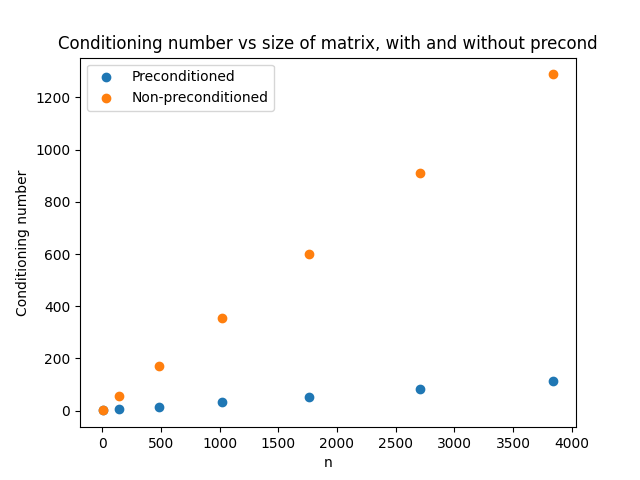
\includegraphics[width=0.8\textwidth]{../images/conditioning_test.png}
	\end{figure}

\end{frame} 


\begin{frame}{Results (iterations)}
\begin{figure}
	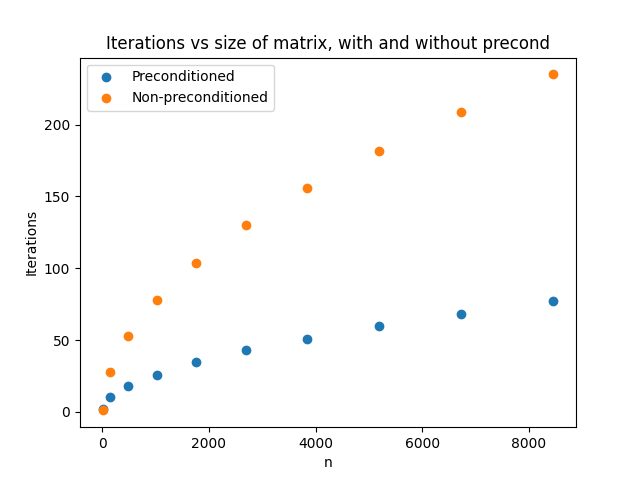
\includegraphics[width=0.8\textwidth]{../images/iterations_test.png}
\end{figure}
\end{frame}

\begin{frame}{Results (residual)}
\begin{figure}
	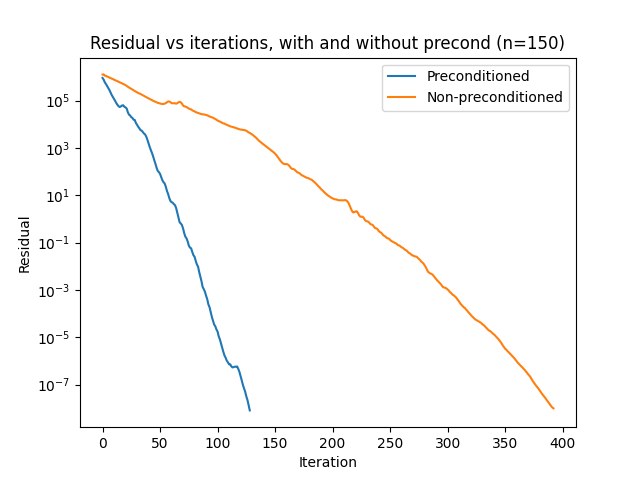
\includegraphics[width=0.8\textwidth]{../images/residual_test.png}
\end{figure}
\end{frame}

\begin{frame}{Results (time)}
\begin{figure}
	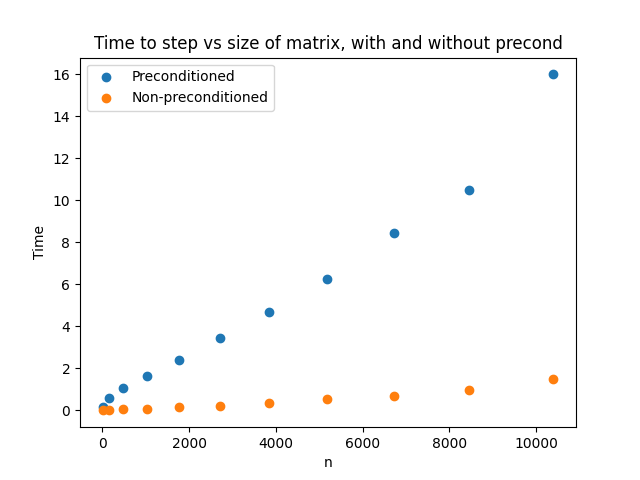
\includegraphics[width=0.8\textwidth]{../images/time_test.png}
\end{figure}
\end{frame}



%%%%%%%%%%%%%%%%%%%%%%%%%%%%%%%%%%%%%%%%%%%%%%%%%%%%%%%%%%%%%%%%
%					References
%%%%%%%%%%%%%%%%%%%%%%%%%%%%%%%%%%%%%%%%%%%%%%%%%%%%%%%%%%%%%%%%

\begin{frame}


%\bibliography{pointwise_refrences}
%\bibliographystyle{plain}
\vspace{0mm}

{\scriptsize
\begin{thebibliography}{10}

\bibitem{A}
Shmuel Agmon. 
\newblock {\em }Princeton University Press, Princeton, NJ; University of Tokyo Press, Tokyo, 1982.

\bibitem{BFS}
Volker Bach, J\"{u}rg Fr\"{o}hlich, and Israel~Michael Sigal.
\newblock {\em Comm. Math. Phys.}, 207(2):249--290, 1999.

\bibitem{DHSV78}
P.~Deift, W.~Hunziker, B.~Simon, and E.~Vock.
\newblock {\em Comm. Math. Phys.}, 64(1):1--34, 1978/79.

\bibitem{G}
M.~Griesemer.
\newblock {\em J. Funct. Anal.}, 210(2):321--340, 2004.

\bibitem{HiHi2010}
Takeru Hidaka and Fumio Hiroshima.
\newblock {\em Rev. Math. Phys.}, 22(10):1181--1208, 2010.

\bibitem{Hi14}
Fumio Hiroshima.
\newblock {\em Adv. Math.}, 259:784--840, 2014.

\bibitem{Hiro2019}
Fumio Hiroshima.
\newblock In {\em Analysis and operator theory}, volume 146 of {\em Springer
  Optim. Appl.}, pages 225--250. Springer, Cham, 2019.
\vspace{-1mm}
\bibitem{HiMa22}
Fumio Hiroshima and Oliver Matte.
\newblock {\em Rev. Math. Phys.}, 34(2):Paper No. 2250002, 84, 2022.

\bibitem{M16}
Oliver Matte.
\newblock {\em Rev. Math. Phys.}, 28(5):1650011, 90, 2016.
\vspace{-1mm}
\bibitem{S79}
Barry Simon.
\newblock {\em J. Functional Analysis}, 32(1):97--101, 1979.

\end{thebibliography}
}

\end{frame}





%\begin{frame}{References}
%\bibliography{pointwise_refrences}
%\bibliographystyle{plain}
%\end{frame}





\end{document}












%----------------------------------------------------------------------------------------
%   Content (end)
%----------------------------------------------------------------------------------------
